\chapter{Conclusion}
\label{chap-conclusion}

In this chapter, we present some additional problems related to universality. As remarked in Chapter~\ref{chap-introduction}, each $n$-structure considered in this work contains at most $\binom{n}{m}$ many $m$-structures, as any substructure of size $m$ corresponds to a subset of entries of size $m$. One may ask more generally, ``what is the maximum number of $m$-structures that an $n$-structure may contain?'' In~\cite{bevan:prolific-permut:}, Bevan, Homberger, and Tenner prove there are $n$-permutations that attain the above binomial bound, meaning they contain $\binom{n}{m}$ many $m$-permutations, if and only if $n \ge \ceil{(n-m)^2/2 + 2(n-m) + 1}$.  Focusing on permutations, let $\Cont(n,m)$ denote the maximum number of $m$-permutations that any $n$-permutation contains. Figure~\ref{fig-perm-max-contain} displays known values of $\Cont(m+k,m)$ for small $m$ and $k$. The cells with dark gray backgrounds contain values where $\Cont(m+k,m) = m!$, meaning there are $m$-universal permutations of size $m+k$. The cells with white backgrounds contain values so that $\Cont(m+k,m) = \binom{m+k}{m}$. We are grateful to Axel Bacher~[private communication] for computing many of these values.

\begin{figure}[ht]
\captionsetup{justification=centering}
    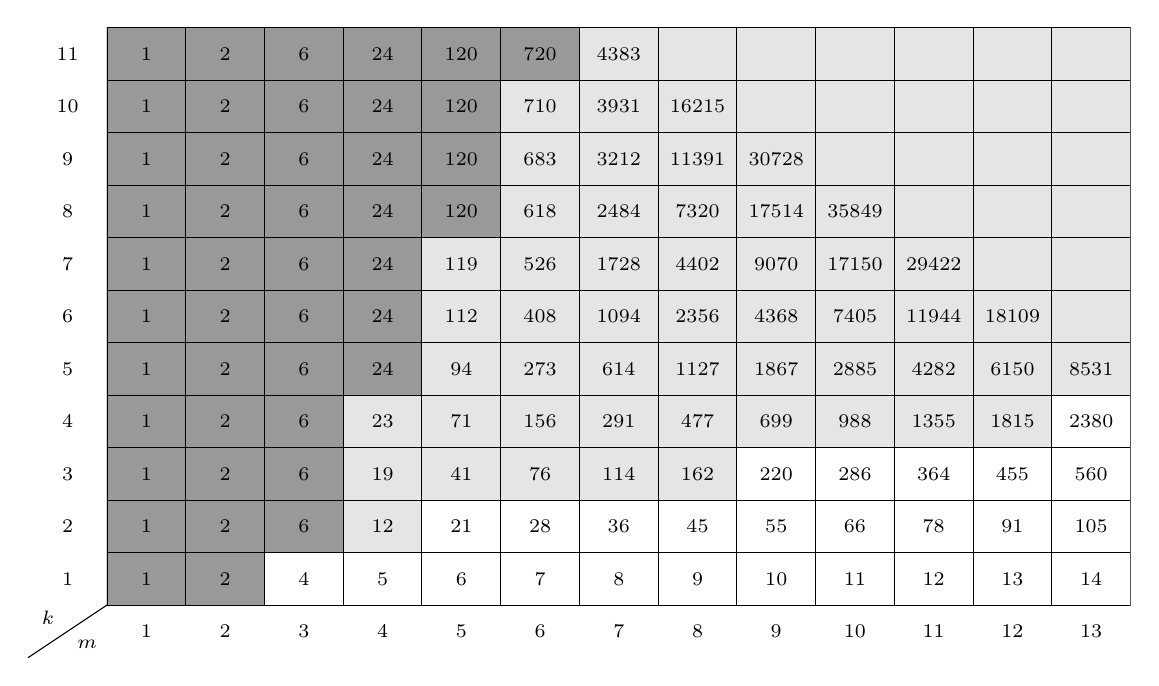
\begin{tikzpicture}[xscale = 1.0, yscale={2/3}]
        \def\height{11}
        \def\width{13}

        \draw[line cap = round] (-0.5,-0.5) -- (0.5,0.5);
        \node at (0.25,-0.25) {$\scriptstyle m$};
        \node at (-0.25,0.25) {$\scriptstyle k$};

        \foreach \x in {1,2,...,\width} {
            \node at (\x, 0) {$\scriptstyle \x$};
        }
        \foreach \y in {1,2,...,\height} {
            \node at (0, \y) {$\scriptstyle \y$};
        }
        \begin{scope}
            \clip (0.5,0.5) rectangle ++(\width,\height);
            \fill[fill=gray!20] (0.5,0.5) rectangle ++(\width,\height);
            
            % DARK GRAY
            \path[fill=gray!80] (0.5,0.5)
                -| ++(2,1)
                -| ++(1,3)
                -| ++(1,3)
                -| ++(1,3)
                -| ++(1,6)
                -| cycle;
            
            % WHITE
            % Bevan, Homberger, Tenner
            \path[fill=white] ( 0.5, 0.5)
                |- ++(2,0)
                |- ++(2,1)
                |- ++(4,1)
                |- ++(4,1)
                |- ++(6,1)
                |- cycle;

            \draw[shift={(0.5,0.5)}, black] (0,0) grid (\width,\height);

            % Known values:
            \foreach \val [count=\x] in {1, 2, 4,  5,   6,   7,    8,     9,    10,    11,    12,    13,   14,   15} {\node at (\x, 1) {$\scriptstyle\val$}; }
			\foreach \val [count=\x] in {1, 2, 6, 12,  21,  28,   36,    45,    55,    66,    78,    91,  105,  120} {\node at (\x, 2) {$\scriptstyle\val$}; }
			\foreach \val [count=\x] in {1, 2, 6, 19,  41,  76,  114,   162,   220,   286,   364,   455,  560,  680} {\node at (\x, 3) {$\scriptstyle\val$}; }
			\foreach \val [count=\x] in {1, 2, 6, 23,  71, 156,  291,   477,   699,   988,  1355,  1815, 2380, 3060} {\node at (\x, 4) {$\scriptstyle\val$}; }
			\foreach \val [count=\x] in {1, 2, 6, 24,  94, 273,  614,  1127,  1867,  2885,  4282,  6150, 8531,     } {\node at (\x, 5) {$\scriptstyle\val$}; }
			\foreach \val [count=\x] in {1, 2, 6, 24, 112, 408, 1094,  2356,  4368,  7405, 11944, 18109,     ,     } {\node at (\x, 6) {$\scriptstyle\val$}; }
			\foreach \val [count=\x] in {1, 2, 6, 24, 119, 526, 1728,  4402,  9070, 17150, 29422,      ,     ,     } {\node at (\x, 7) {$\scriptstyle\val$}; }
			\foreach \val [count=\x] in {1, 2, 6, 24, 120, 618, 2484,  7320, 17514, 35849,      ,      ,     ,     } {\node at (\x, 8) {$\scriptstyle\val$}; }
			\foreach \val [count=\x] in {1, 2, 6, 24, 120, 683, 3212, 11391, 30728,      ,      ,      ,     ,     } {\node at (\x, 9) {$\scriptstyle\val$}; }
			\foreach \val [count=\x] in {1, 2, 6, 24, 120, 710, 3931, 16215,      ,      ,      ,      ,     ,     } {\node at (\x,10) {$\scriptstyle\val$}; }
			\foreach \val [count=\x] in {1, 2, 6, 24, 120, 720, 4383,      ,      ,      ,      ,      ,     ,     } {\node at (\x,11) {$\scriptstyle\val$}; }
			\foreach \val [count=\x] in {1, 2, 6, 24, 120, 720,     ,      ,      ,      ,      ,      ,     ,     } {\node at (\x,12) {$\scriptstyle\val$}; }
			\foreach \val [count=\x] in {1, 2, 6, 24, 120, 720,     ,      ,      ,      ,      ,      ,     ,     } {\node at (\x,13) {$\scriptstyle\val$}; }
			\foreach \val [count=\x] in {1, 2, 6, 24, 120, 720,     ,      ,      ,      ,      ,      ,     ,     } {\node at (\x,14) {$\scriptstyle\val$}; }
        \end{scope}
    \end{tikzpicture}
\caption{An array of known values of $\Cont(m+k,m)$ for small values of $m, k$.}
\label{fig-perm-max-contain}
\end{figure}

Given a set of structures $\S$, and let $\Cont_{\S}(n, m)$ denote the maximum number of $\S_m$-structures that any $n$-structure may contain. Likewise, let $\Cont_{\S}^p(n, m)$ denote the maximum number of $\S_m$-structures that any $\S_n$-structure may contain. As a case study, consider the poset $\T$ of words over the two-letter alphabet $\{\worda, \wordb\}$ under the subword ordering. In this case, we may provide an exact formula for the maximum number of words of size $m$ that any word in $\T_n$ may contain.

\begin{proposition}
\label{prop-word-max-contain}
For all $n, m$, the maximum number of $m$-words contained in a $\T_n$-word is
\[
    \Cont_{\T}(n,m) 
    = 
    \sum_{\ell = 0}^{n-m} \binom{m}{\ell}.
\]
\end{proposition}
Before proving Proposition~\ref{prop-word-max-contain}, we note that the formula provided equals $2^{m}$ precisely when $n \ge 2m$, which is implied by Theorem~\ref{prop-word-universal}.
\begin{proof}
To begin, we obtain an recursive formula for the number of $m$-words contained in a word $w$ of size $n$ for $n > m$. If $w$ contains only $\worda$ or only $\wordb$, then $w$ contains only the constant word of size $m$. Otherwise, $w$ contains both $\worda$ and $\wordb$, and without loss of generality we can assume that $w$ ends in $\worda$ and write $w = w_0 \wordb \worda^k$. 

For each word $v$ that $w$ contains that ends in $\wordb$, there is some embedding of $v$ into $w$ that places the final letter of $v$ into the final $\wordb$ of $w$, and thus the set of $m$-words contained in $w$ that end in $\wordb$ is in bijection with the set of $(m-1)$-words contained in $w_0$. Likewise, the set of $m$-words contained in $w$ that end in $\worda$ is in bijection with the set of $(m-1)$-words contained in $w_0 \wordb \worda^{k-1}$. % Let $\cont_w(m)$ denote the number of $m$-words contained in $w$. 
We have shown that 
\[
    \binom{\text{$\#$ of $m$-words}}{\text{contained in $w$}}
    =
    \binom{\text{$\#$ of $(m-1)$-words}}{\text{contained in $w_0$}}
    +
    \binom{\text{$\#$ of $(m-1)$-words}}{\text{contained in $w_0 \wordb \worda^{k-1}$}}.
\]
% \[
%     \cont_{w}(m) 
%     = 
%     \cont_{w_0}(m-1) + \cont_{w_0 \wordb \worda^{k-1}}(m-1).
% \]

This formula implies an upper bound on the quantity $\Cont_{\T}(n,m)$. As $w_0$ has size at most $n-2$ and $w_0 \wordb \worda^{k-1}$ has size at most $n-1$, we have
\begin{align*}
    \binom{\text{$\#$ of $m$-words}}{\text{contained in $w$}}
        &= \binom{\text{$\#$ of $(m-1)$-words}}{\text{contained in $w_0$}}
         + \binom{\text{$\#$ of $(m-1)$-words}}{\text{contained in $w_0 \wordb \worda^{k-1}$}} \\
        &\le \Cont_{\T}(n-2,m-1) + \Cont_{\T}(n-1,m-1)
\end{align*}
for all words $w$. Thus the maximum number of $m$-words contained among all words in $\T_n$ obeys this bound as well, and thus we have
\[
    \Cont_{\T}(n,m)
    \le
    \Cont_{\T}(n-2,m-1) + \Cont_{\T}(n-1,m-1).
\]

To establish equality, we exhibit a word $w_n$ of size $n$ that attains this upper bound. For each $n \ge 0$, let $w_n$ be the word of size $n$ wherein each letter in an odd position is $\worda$ and each letter in an even position is $\wordb$, e.g. $w_0 = \varepsilon$, $w_1 = \worda$, $w_2 = \worda \wordb$, $w_3 = \worda \wordb \worda$, and so on. Let $\cont(n, m)$ denote the number of $m$-words contained in $w_n$.

We claim that for all $n$, $\cont(n, m) = \Cont_{\T}(n, m)$, and proceed by induction on $m$. For our base case of $m = 0$, every word contains the unique empty word, so $\cont(n, 0) = \Cont_{\T}(n, 0) = 1$. Now, assume that for all $n$ we have $\cont(n, m') = \Cont_{\T}(n, m')$ for all $m' < m$. By the recursive formula at the beginning of this proof, we have
\begin{align*}
    \cont(n, m)
        &= \cont(n-1, m-1) + \cont(n-2, m-1) \\
        &= \Cont_{\T}(n-1, m-1) + \Cont_{\T}(n-2, m-1) \\
        &\ge \Cont_{\T}(n,m).
\end{align*}
As $w_n$ is a word of size $n$, we have that $\cont(n,m) \le \Cont_{\T}(n,m)$, and thus we have equality:
\[
    \cont(n, m)
    =
    \Cont_{\T}(n,m)
    =
    \Cont_{\T}(n-1,m-1) + \Cont_{\T}(n-1,m-1).
\]

It only remains to show that for all $n$,
\[
    \Cont_{\T}(n,m)
    = 
    \sum_{\ell = 0}^{n-m} \binom{m}{\ell},
\]
which we show by induction on $m$.

For all $n$, we have $\Cont_{\T}(n,0) = \binom{0}{0} + \binom{0}{1} + \cdots + \binom{0}{n-m} = 1 + 0 + \cdots + 0 = 1$. Fix $m \ge 1$, and assume that the statement holds for all values less than $m$. Then we have
\begin{align*}
    \Cont_{\T}(n,m) 
        &= \Cont_{\T}(n-1,m-1) + \Cont_{\T}(n-2,m-1) \\
        &= \sum_{\ell = 0}^{n-m} \binom{m-1}{\ell} + \sum_{\ell = 0}^{n-m-1} \binom{m-1}{\ell} \\
        &= \binom{m-1}{0} + \sum_{\ell = 0}^{n-m-1} \left[ \binom{m-1}{\ell+1} + \binom{m-1}{\ell} \right] \\
        &= \binom{m}{0} + \sum_{\ell = 0}^{n-m-1} \binom{m}{\ell+1} \\
        &= \binom{m}{0} + \sum_{\ell = 1}^{n-m} \binom{m}{\ell} \\
        &= \sum_{\ell = 0}^{n-m} \binom{m}{\ell},
\end{align*}
as desired.
\end{proof}

Values of $\Cont_{\T}(m+k,m)$ for small values of $m$ and $k$ are displayed in Figure~\ref{fig-max-contain-words}. The recurrence proven in the proof of Proposition~\ref{prop-word-max-contain} may be interpreted in this context as ``the value in a cell is equal to the sum of the values in the cells immediately to its west and to its south-west''. As in Figure~\ref{fig-perm-max-contain}, the cells with dark gray backgrounds correspond to universality, and the cells with white backgrounds contain values so that $\Cont_{\T}(m+k,m) = \binom{m+k}{m}$.

\begin{figure}[ht]
\captionsetup{justification=centering}
\begin{tikzpicture}[xscale=1, yscale={2/3}]
    \def\height{10}
    \def\width{10}
    
    \draw[line cap = round] (-0.5,-0.5) -- (0.5,0.5);
    \node at (0.25,-0.25) {$\scriptstyle m$};
    \node at (-0.25,0.25) {$\scriptstyle k$};
    
    \foreach \x in {1,2,...,\width} {
        \node at (\x, 0) {$\scriptstyle \x$};
    }
    \foreach \y in {1,2,...,\height} {
        \node at (0, \y) {$\scriptstyle \y$};
    }
    
    \begin{scope}
        \clip (0.5,0.5) rectangle ++(\width,\height);
        \fill[fill=gray!20] (0.5,0.5) rectangle ++(\width,\height);
        
        % White
        \path[fill=white] ( 0.5, 0.5)
                |- ++(10,1) |- cycle;
        
        % Dark gray
        \path[fill=gray!80] (0.5,1.5)
                -| ++(1,0)
                -| ++(1,1) -| ++(1,1) -| ++(1,1) -| ++(1,1)
                -| ++(1,1) -| ++(1,1) -| ++(1,1) -| ++(1,1)
                -| ++(1,1) -| cycle;
        
        % Hatched dark gray
        \path[pattern = north east lines, pattern color = gray!80] (0.5, 0.5) 
            |- ++(1,1)
            |- cycle;
    
        \draw[shift={(0.5,0.5)}, black] (0,0) grid (\width,\height);

        % \foreach \val [count=\x] in { 1, 1,  1,  1,  1,  1,  1,   1,   1,   1} {\node at ( 0,\x) {$\scriptstyle\val$};}
        \foreach \val [count=\x] in { 2, 2,  2,  2,  2,  2,  2,   2,   2,   2} {\node at ( 1,\x) {$\scriptstyle\val$};}
        \foreach \val [count=\x] in { 3, 4,  4,  4,  4,  4,  4,   4,   4,   4} {\node at ( 2,\x) {$\scriptstyle\val$};}
        \foreach \val [count=\x] in { 4, 7,  8,  8,  8,  8,  8,   8,   8,   8} {\node at ( 3,\x) {$\scriptstyle\val$};}
        \foreach \val [count=\x] in { 5,11, 15, 16, 16, 16, 16,  16,  16,  16} {\node at ( 4,\x) {$\scriptstyle\val$};}
        \foreach \val [count=\x] in { 6,16, 26, 31, 32, 32, 32,  32,  32,  32} {\node at ( 5,\x) {$\scriptstyle\val$};}
        \foreach \val [count=\x] in { 7,22, 42, 57, 63, 64, 64,  64,  64,  64} {\node at ( 6,\x) {$\scriptstyle\val$};}
        \foreach \val [count=\x] in { 8,29, 64, 99,120,127,128, 128, 128, 128} {\node at ( 7,\x) {$\scriptstyle\val$};}
        \foreach \val [count=\x] in { 9,37, 93,163,219,247,255, 256, 256, 256} {\node at ( 8,\x) {$\scriptstyle\val$};}
        \foreach \val [count=\x] in {10,46,130,256,382,466,502, 511, 512, 512} {\node at ( 9,\x) {$\scriptstyle\val$};}
        \foreach \val [count=\x] in {11,56,176,386,638,848,968,1013,1023,1024} {\node at (10,\x) {$\scriptstyle\val$};}
        
    \end{scope}
    
\end{tikzpicture}
\caption{An array containing the values $\Cont_{\T}(m+k, m)$ for small values of $m$ and $k$.}
\label{fig-max-contain-words}
\end{figure}

By the isomorphism between the poset of words over a two-letter alphabet and the poset $\W$ of non-empty wedge permutations in Proposition~\ref{prop-perm-wedge-isomorphism}, the maximum number of $\W_m$-permutations that any $\W_n$-permutation may contain is $\sum_{\ell = 0}^{n-m} \binom{m-1}{\ell}$. Computation suggests that the maximum number of $\W_m$-permutations contained by \emph{any} permutation of size $n$ is $\sum_{\ell = 0}^{n-m} \binom{m-1}{\ell}$ as well.

\begin{conjecture}
\label{conj-max-contain-w}
For all $m$ and $n$, the maximum number of $\W_m$-permutations contained by any permutation of size $n$ is
\[
    \sum_{\ell = 0}^{n-m} \binom{m-1}{\ell}.
\]
\end{conjecture}